% Standalone vector figure extracted from manuscript.tex.
% Rebuild all figures from the project root: bash tkz/build.sh
\documentclass[tikz,border=2pt,class=IEEEtran]{standalone}
\usepackage{amsmath,amssymb,amsfonts}
\usepackage{xcolor}
\usetikzlibrary{positioning,arrows.meta,calc,backgrounds}

% Match the manuscript's IEEE Access text and math font settings.
\renewcommand{\textbf}[1]{{\fontseries{b}\selectfont #1}}
\renewcommand{\textit}[1]{{\itshape #1}}
\makeatletter
\AtBeginDocument{%
  \fontencoding{T1}\rmfamily\fontseries{m}\fontsize{10}{12}\selectfont
  \gdef\operator@encoding{T1}%
  \gdef\encodingdefault{T1}}
\makeatother

% ---- shared palette for review figures ----
\definecolor{cVLA}{HTML}{34618E}   % VLA lane / policy blue
\definecolor{cWM}{HTML}{9E4A3F}    % world-model lane
\definecolor{cCONV}{HTML}{5E4B8B}  % convergence purple
\definecolor{cGood}{HTML}{3A7D44}  % verified green
\definecolor{cWarn}{HTML}{B07A2A}  % caution amber
\definecolor{cPale}{HTML}{F2F0EA}  % pale panel fill
\tikzset{
  fnode/.style={draw=black!55, fill=white, rounded corners=1.5pt,
                inner sep=2.5pt, align=center, font=\fontsize{8}{9.5}\selectfont},
  flane/.style={draw=none, rounded corners=2pt, inner sep=3pt,
                align=center, font=\fontsize{8}{9.5}\selectfont\bfseries, text=white},
  farr/.style={-{Stealth[length=2mm]}, thick, black!60},
}


\newcommand{\figfont}{\fontsize{8}{9.5}\selectfont}

\begin{document}

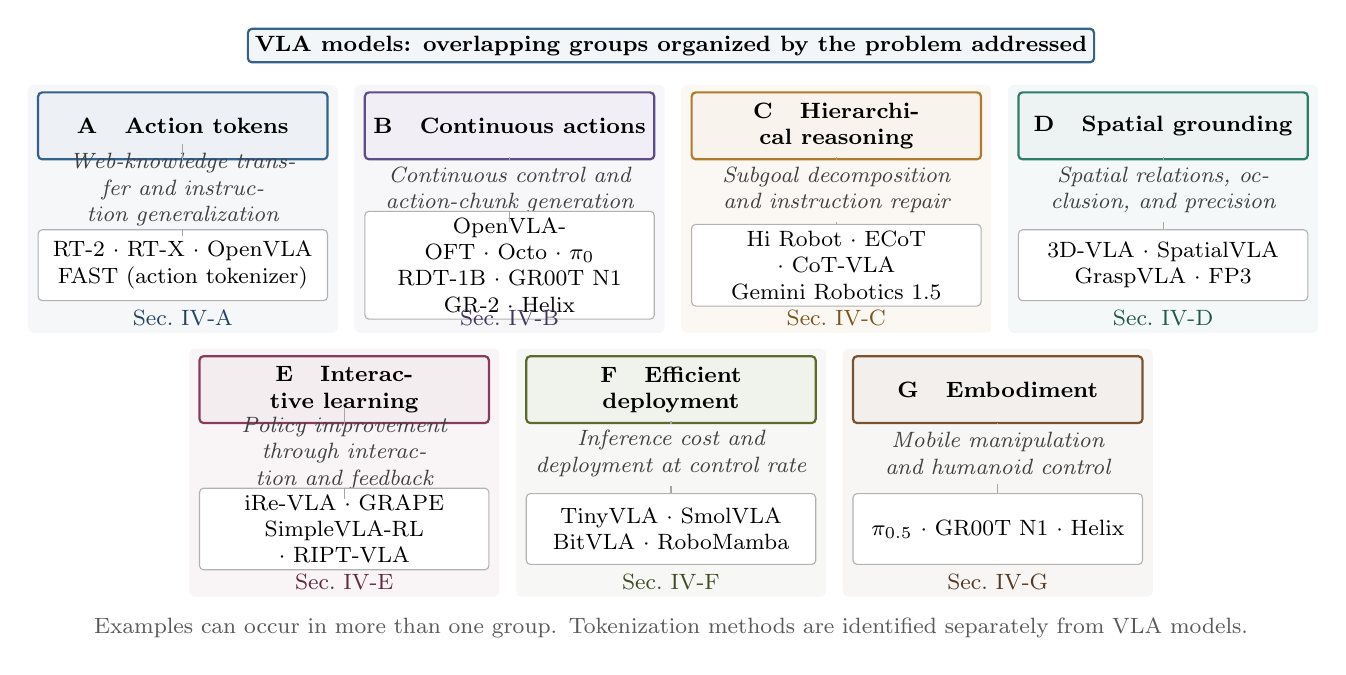
\begin{tikzpicture}[font=\figfont]
\colorlet{gA}{cVLA}\colorlet{gB}{cCONV}\colorlet{gC}{cWarn}
\definecolor{gD}{HTML}{2E7D6B}\definecolor{gE}{HTML}{8A3B5C}
\definecolor{gF}{HTML}{5B6B2F}\definecolor{gG}{HTML}{7A5230}
\node[fnode,draw=cVLA,thick,fill=cVLA!6,font=\figfont\bfseries] at (8.2,.6)
 {VLA models: overlapping groups organized by the problem addressed};
% Wider cards keep the connector paths outside all text.
\foreach \x/\y/\cc/\head/\problem/\models/\sec in {
 2/0/gA/{A\quad Action tokens}/{Web-knowledge transfer and instruction generalization}/{RT-2 $\cdot$ RT-X $\cdot$ OpenVLA\\FAST (action tokenizer)}/{IV-A},
 6.15/0/gB/{B\quad Continuous actions}/{Continuous control and action-chunk generation}/{OpenVLA-OFT $\cdot$ Octo $\cdot$ $\pi_0$\\RDT-1B $\cdot$ GR00T N1\\GR-2 $\cdot$ Helix}/{IV-B},
 10.3/0/gC/{C\quad Hierarchical reasoning}/{Subgoal decomposition and instruction repair}/{Hi Robot $\cdot$ ECoT $\cdot$ CoT-VLA\\Gemini Robotics 1.5}/{IV-C},
 14.45/0/gD/{D\quad Spatial grounding}/{Spatial relations, occlusion, and precision}/{3D-VLA $\cdot$ SpatialVLA\\GraspVLA $\cdot$ FP3}/{IV-D},
 4.05/-3.35/gE/{E\quad Interactive learning}/{Policy improvement through interaction and feedback}/{iRe-VLA $\cdot$ GRAPE\\SimpleVLA-RL $\cdot$ RIPT-VLA}/{IV-E},
 8.2/-3.35/gF/{F\quad Efficient deployment}/{Inference cost and deployment at control rate}/{TinyVLA $\cdot$ SmolVLA\\BitVLA $\cdot$ RoboMamba}/{IV-F},
 12.35/-3.35/gG/{G\quad Embodiment}/{Mobile manipulation and humanoid control}/{$\pi_{0.5}$ $\cdot$ GR00T N1 $\cdot$ Helix}/{IV-G}}{
 \begin{scope}[shift={(\x,\y)}]
 \fill[\cc!5,rounded corners=2pt] (-1.97,-3.05) rectangle (1.97,.1);
 \node[fnode,draw=\cc,thick,fill=\cc!9,text width=35mm,minimum height=8.5mm,font=\figfont\bfseries] (h) at (0,-.42) {\head};
 \node[align=center,text width=35mm,font=\figfont\itshape,text=black!75] (p) at (0,-1.23) {\problem};
 \node[fnode,draw=black!30,text width=35mm,minimum height=9mm] (m) at (0,-2.19) {\models};
 \draw[black!35] (h.south)--(p.north);
 \draw[black!35] (p.south)--(m.north);
 \node[text=\cc!70!black] at (0,-2.86) {Sec.~\sec};
 \end{scope}}
\node[text=black!65,align=center,text width=150mm] at (8.2,-6.8)
 {Examples can occur in more than one group. Tokenization methods are identified separately from VLA models.};
\end{tikzpicture}
\end{document}
